\documentclass[a4paper, 10pt]{article}
\usepackage[margin = 1in]{geometry}
\usepackage{amsmath}
\usepackage{tabularx}
\usepackage{framed}
\setlength{\parindent}{0em}
\newcolumntype{L}{>{\arraybackslash}m{10cm}}
\newcolumntype{T}{>{\arraybackslash}m{6cm}}
\usepackage{graphicx}
\usepackage{pdfpages}

\begin{document}

\section*{Topic 14 - Current of electricity}

\section{Electric Current and charge}

\subsection{Electric Current}
\begin{framed}
   \textbf{Electric current} is defined as the rate of flow of charge
   \[
   I = \frac{dQ}{dt}
   \]
   The S.I. unit for current is Ampere
\end{framed}	

\subsection{Charge}
\begin{framed}
   Electical charge is a fundamental property of matter which causes a charged particle to experience a force when placed in an electric field. \\

   When a current $I$ flows through a cross-section of a conductor for duration $t$, the amount of \textbf{electrical charge} passing through is given by
   \[
   Q = It
   \]

   One \textbf{coulomb} is defined as the amount of charge that passes through a point in one second due to a current of one ampere
   
\end{framed}	

\subsection{Drift velocity}
For a conductor with cross sectional area $A$ and $n$ charge carriers per unit volume, and a current $I$ \\

In the time interval $\Delta t$ , each charge moves a distance of
\[
   v_D( \Delta T), \text{ where $v_D$ is the drift velocity}
\]

The number of charge carriers passing through a point in duration $\Delta t$ is thus
\[
nA v_D \Delta t
\]

total charge passing through is 
\[
nA v_d \Delta t q
\]
current is thus
\[
I = \frac{nAv_d \Delta t}{\Delta t} = nAv_Dq 
\]



\section{Potential difference}

\begin{framed}
   The \textbf{potential difference} between two points in a circuit is defined as the amount of electrical energy per unit charge that is converted to other forms of energy when charge passes from one point to another
   \[
   V = \frac{W}{Q}
   \]

   The SI units for p.d. is volt \\
   one volt is the potential difference between two points when one joule of electrical energy is converted to other forms of energy as one coulomb of charge passes from one point to another
\end{framed}	

\section{Electromotive Force}
\begin{framed}
   the \textbf{electromotive force} of a source is defined as the amount of electrical energy per unit charge that is converted from other forms of energy when charge passes through the source
   \[
   E = \frac{W}{Q}
   \]
\end{framed}	

\section{Resistance and resistivity}
\begin{framed}
   The \textbf{resistance} of a circuit component is defined as the ratio of the potential difference across it to the current flowing through it
   \[
   R = \frac{V}{I}
   \]

   one \textbf{$\Omega$} is the resitance of a conductor when a potential difference of one volt across it causes a current of one ampere to flow through
\end{framed}	

\subsection{Ohm's law}
\begin{framed}
   \textbf{Ohm's law} states that the potential difference across a conductor is proportial to the electric current passing through it, provided that its temperature remains constant
\end{framed}	

\subsection{Resistivity $\rho$}
The resistance of a unifom conductor is 
\begin{itemize}
   \item directly proportional to its length, $l$ 
   \item inversely proportional to its cross sectional area, $A$ 
\end{itemize}	

hence \[
R \propto \frac{l}{A}
\]

\[
R = \rho \frac{l}{A}
\]

\subsection{Effect of temperature changes}
\begin{itemize}
   \item Effect 1: increase in density of free electrons. More electrons able to break free from atoms, more mobile electrons
   \item Effect 2: lattice ions vibrate faster with greater amplitudes. Electrons lose KE to fixed ions during collision, hence emperature increases. Ions then vibrate faster with greater amplitudes, making it more difficult for electrons to pass through the lattice
\end{itemize}	

\begin{center}
   \begin{tabular}{c | T | T}
      materials & metallic conductors & semiconductors - NTC thermistors \\
      \hline
      Effect 1 & Electrons are already mobile at room temperature. No appreciable increase in number of conducting electrons & Semiconductors are poor conductors at low temperatures. Conductivity increases significantly with temperature \\
      \hline
      Effect 2 & Significantly greater vibration of lattice ions, resistance increases & Significantly greater vibration of lattice ions.\\
      \hline
      Change in resistance & Effect 1 insignificant, effect 2 is present, resistance increases with temperature & Effect 1 more significant than effect 2. Resistance decreases with temperature \\ & &  \\
                           &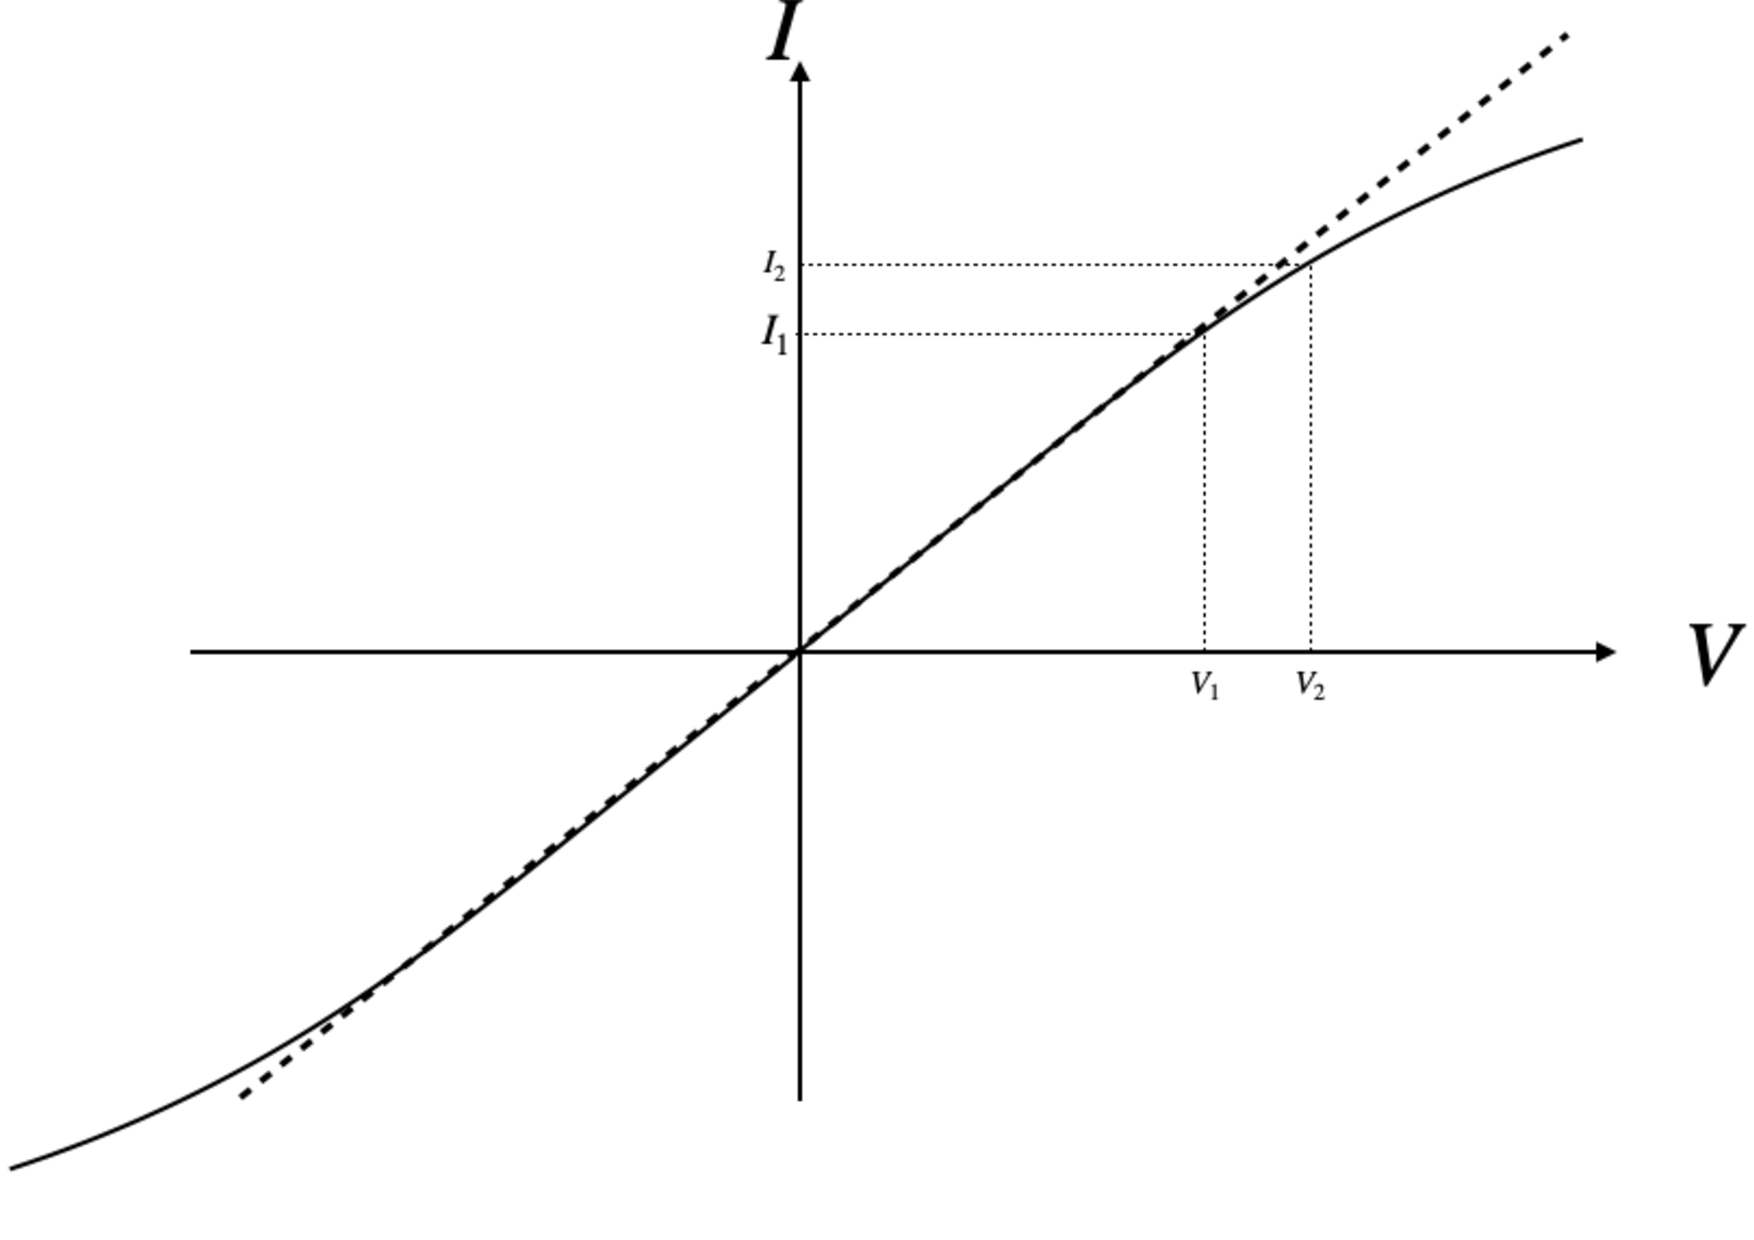
\includegraphics[trim = 50 50 50 50, width=6cm]{figures/2.pdf} & 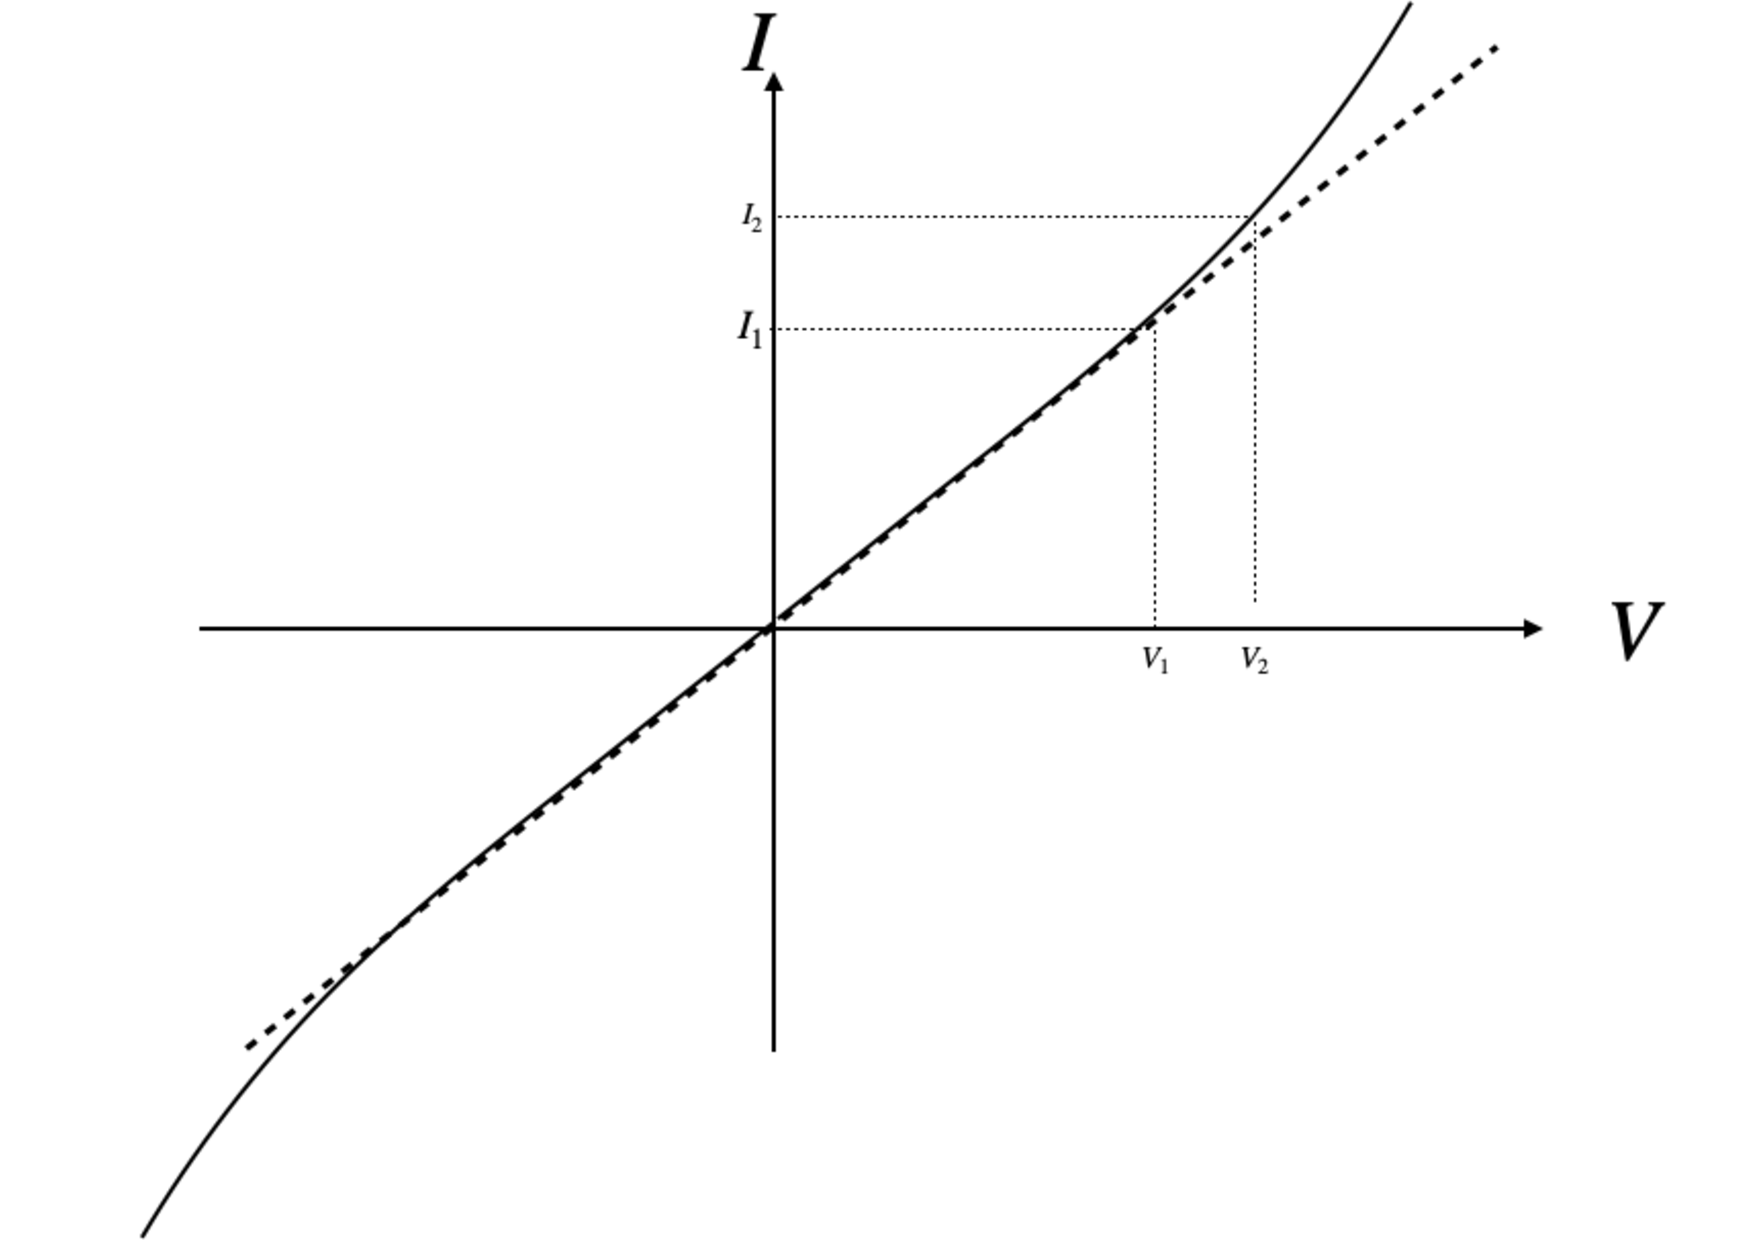
\includegraphics[trim = 50 50 50 50, width=6cm]{figures/3.pdf}   \\
   \end{tabular}
\end{center}

\section{Electrical power}
When a charge $Q$ moves through a p.d. $V$, the amount of electrical energy converted to other forms is
\[
W = QV
\]
the rate of energy convertion is
\[
   P = \frac{dW}{dt} = \frac{d(QV)}{dt} = \frac{dQ}{dt}V = IV
\]

\subsection{Power of an ideal source}
For an ideal source, work done is
\[
W = QE
\]
The power supplied is
\[
P = \frac{dW}{dt} = \frac{dQ}{dt}E
\]
\[
P = IE
\]

\subsection{Power dissipated by a resistor}
The p.d. across a resistor is
\[
V = IR
\]
The rate of energy dissipation is 
\[
P = IV = I^2R = \frac{V^2}{R}
\]

\section{Internal resistance of a source}
For a real battery with internal resistance $r$ connected to a circuit with resistor $R$  \\

The power supplied by source is 
\[
P_s = IE
\]
Power dissipated in internal resistance is 
\[
P_r = I^2r
\]
Power dissipated in external load is
\[
P_R = I^2R
\]

By principle of conservation of energy
\[
P_S = P_r + P_R
\]
\[
IE = I^2 r + I^2R
\]

\[
   E = I(r + R)
\]

\[
E = Ir + V_R
\]

\[
V_R = E - Ir
\]

Hence terminal p.d. $V$ decreases with increasing $I$ 

\subsection{Power output and max power theorem}
since
\[
   E = I(r + R) \\
\]
\[
I = \frac{E}{r+R}
\]
heat transferred to external load $R$ is
\[
   P_R = I^2 R = \left( \frac{E}{r + R} \right)^2 R 
\]
\[
   P_R = \frac{E^2R}{(r+R)^2}
\]

Max power delivered to external load $R$ can be found by taking the derivative
\begin{align*}
   \frac{dP_R}{dR} &= 0 \\
0 &= \frac{E^2 (r+R) - 2E^2 R}{(r+R)^3} \\
E^2(r+R) - 2E^2R &= 0 \\
r + R - 2R &= 0 \\
r &= R 
\end{align*}	

Hence a source of emf delivers the maximum amount of power to an external load when the resistance of the load is equal to the internal resistance of the source




\end{document}	
